% Diagram
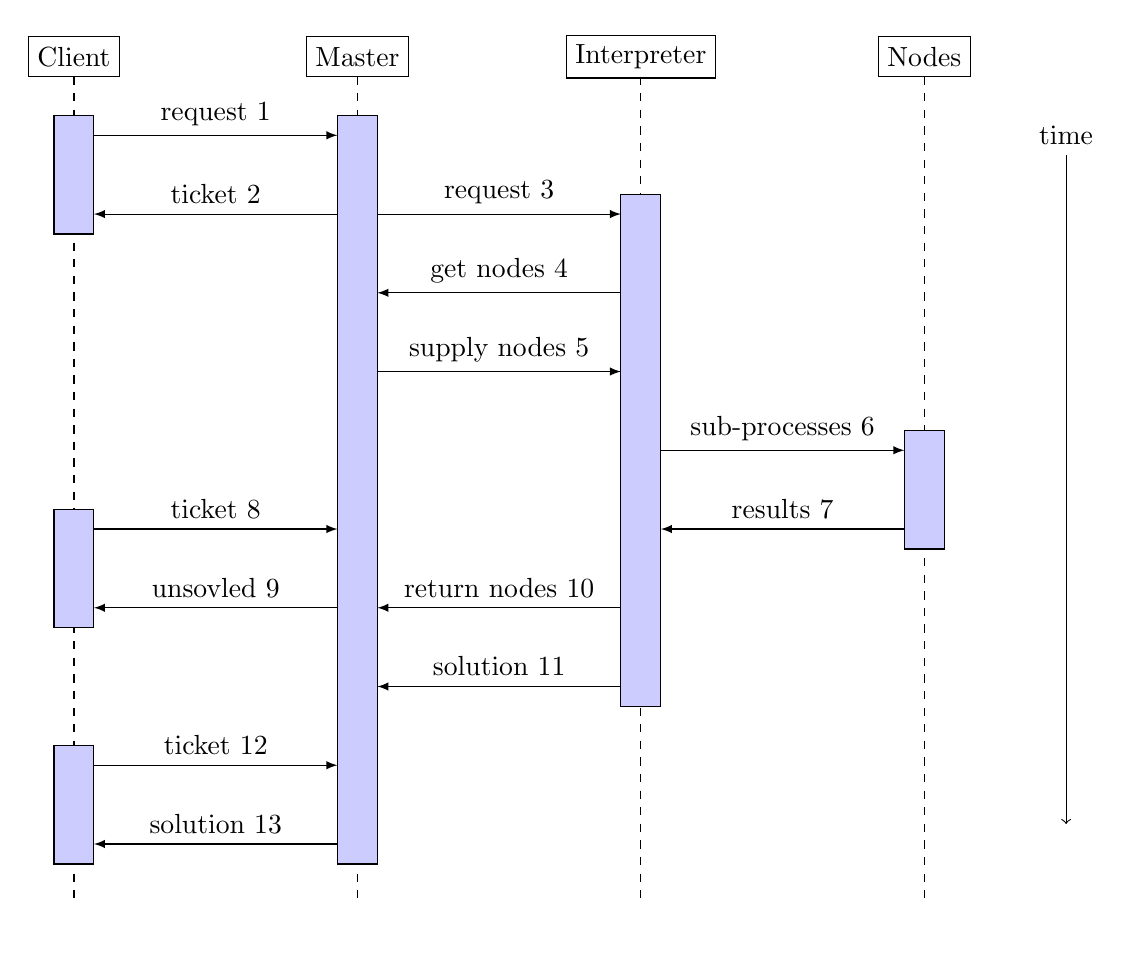
\begin{tikzpicture}[every node/.style={font=\normalsize,minimum height=0.5cm,minimum width=0.5cm},]

% Matrix
\node [matrix, very thin,column sep=1.3cm,row sep=0.5cm] (matrix) at (0,0) {
  \node(0,0) (c)  {}; &                       & \node(0,0) (m)  {}; &                       & \node(0,0) (i)  {}; &                       & \node(0,0) (ns) {}; & \\
  \node(0,0) (c0) {}; & \node(0,0) (c0m0) {}; & \node(0,0) (m0) {}; &                       &                     &                       &                     & \node(0,0) (t0) {}; \\
  \node(0,0) (c1) {}; & \node(0,0) (m1c1) {}; & \node(0,0) (m1) {}; & \node(0,0) (m1i1) {}; & \node(0,0) (i1) {}; &                       &                     & \\
  \node(0,0) (c2) {}; &                       & \node(0,0) (m2) {}; & \node(0,0) (i2m2) {}; & \node(0,0) (i2) {}; &                       &                     & \\
  \node(0,0) (c3) {}; &                       & \node(0,0) (m3) {}; & \node(0,0) (m3i3) {}; & \node(0,0) (i3) {}; &                       &                     & \\
  \node(0,0) (c4) {}; &                       & \node(0,0) (m4) {}; &                       & \node(0,0) (i4) {}; & \node(0,0) (i4n4) {}; & \node(0,0) (n4) {}; & \\
  \node(0,0) (c5) {}; & \node(0,0) (c5m5) {}; & \node(0,0) (m5) {}; &                       & \node(0,0) (i5) {}; & \node(0,0) (n5i5) {}; & \node(0,0) (n5) {}; & \\
  \node(0,0) (c6) {}; & \node(0,0) (m6c6) {}; & \node(0,0) (m6) {}; & \node(0,0) (i6m6) {}; & \node(0,0) (i6) {}; &                       &                     & \\
  \node(0,0) (c7) {}; &                       & \node(0,0) (m7) {}; & \node(0,0) (i7m7) {}; & \node(0,0) (i7) {}; &                       &                     & \\
  \node(0,0) (c8) {}; & \node(0,0) (c8m8) {}; & \node(0,0) (m8) {}; &                       & \node(0,0) (i8) {}; &                       &                     & \\
  \node(0,0) (c9) {}; & \node(0,0) (m9c9) {}; & \node(0,0) (m9) {}; &                       & \node(0,0) (i9) {}; &                       & \node(0,0) (n9) {}; & \node(0,0) (t9) {}; \\
  \node(0,0) (cx) {}; &                       & \node(0,0) (mx) {}; &                       & \node(0,0) (ix) {}; &                       & \node(0,0) (nx) {}; & \node(0,0) (tx) {}; \\
};

% Process labels
\fill 
  (c)  node[draw,fill=white] {Client}
  (m)  node[draw,fill=white] {Master}
  (i)  node[draw,fill=white] {Interpreter}
  (ns) node[draw,fill=white] {Nodes}
  (t0) node                  {time};

% Vertical lifelines
\draw [dashed]
  (c)  -- (cx)
  (m)  -- (mx)
  (i)  -- (ix)
  (ns) -- (nx);

\draw [style=->] (t0) -- (t9);

% Blocks
\filldraw[fill=blue!20]
  (c0.north west) rectangle (c1.south east)
  (c5.north west) rectangle (c6.south east)
  (c8.north west) rectangle (c9.south east)
  (m0.north west) rectangle (m9.south east)
  (i1.north west) rectangle (i7.south east)
  (n4.north west) rectangle (n5.south east);

% communication
\draw [-latex] (c0) -- (m0);
\draw [-latex] (m1) -- (c1);
\draw [-latex] (m1) -- (i1);
\draw [-latex] (i2) -- (m2);
\draw [-latex] (m3) -- (i3);
\draw [-latex] (c5) -- (m5);
\draw [-latex] (i4) -- (n4);
\draw [-latex] (m6) -- (c6);
\draw [-latex] (n5) -- (i5);
\draw [-latex] (i6) -- (m6);
\draw [-latex] (i7) -- (m7);
\draw [-latex] (c8) -- (m8);
\draw [-latex] (m9) -- (c9);

\fill
  (c0m0) node[above] {request \smallfigannotation{1}}
  (m1c1) node[above] {ticket \smallfigannotation{2}}
  (m1i1) node[above] {request \smallfigannotation{3}}
  (i2m2) node[above] {get nodes \smallfigannotation{4}}
  (m3i3) node[above] {supply nodes \smallfigannotation{5}}
  (i4n4) node[above] {sub-processes \smallfigannotation{6}}
  (n5i5) node[above] {results \smallfigannotation{7}}
  (c5m5) node[above] {ticket \smallfigannotation{8}}
  (m6c6) node[above] {unsovled \smallfigannotation{9}}
  (i6m6) node[above] {return nodes \smallfigannotation{10}}
  (i7m7) node[above] {solution \smallfigannotation{11}}
  (c8m8) node[above] {ticket \smallfigannotation{12}}
  (m9c9) node[above] {solution \smallfigannotation{13}}
;

\end{tikzpicture}